\documentclass{article}

\usepackage[margin=1.5cm]{geometry} % margins
\usepackage{multicol} % columns
\usepackage{natbib} % references
\usepackage{pgfplots} % plots
\usepackage{tikz} % more plots
\usepackage{float} % layout
\usepackage{array}
\usepackage{algorithm}
\usepackage[noend]{algpseudocode}% http://ctan.org/pkg/algorithm
\usepackage{hyperref}
\usepackage{amssymb}
\usepackage{booktabs}
\usepackage{multirow}
\usepackage{amsmath}

\newcommand*\rot{\rotatebox{90}}
\newcommand{\Lagr}{\mathcal{L}}
\newcolumntype{M}{>{\centering\arraybackslash}m{\dimexpr.5\linewidth-2\tabcolsep}}
\usepgfplotslibrary{groupplots}

\author{Eden Attenborough 100301654 \and Cameron Bateman xxxxxxxxx}
\title{CMP-6035B - Image categorisation I}

\begin{document}

\begin{multicols}{2}

\maketitle
\section{Literature Review}

% \columnbreak
\subsection{Feature Detection \& Description}
Feature detection in computer vision is the process of extracting pieces of information from within an image, typically whether a certain region of the image contains unique properties. These properties can vary but common ones are corners, edges or curves and are commonly referred to as local features.

Feature description in computer vision is a method to describe local properties of an image at pixel coordinates marked via a feature detection algorithm. These methods extract valuable information from the image data and are then commonly stored in a vector, termed a feature vector. 

Features in image processing fall into two categories; global and local features. These two categories vary in their application, with global features typically being used in image retrieval (CBIR \cite{image-retrieval-global-features}), object detection and classification, while local features are commonly used for recognition and identification.

\begin{itemize}
	\item Global features are those which describe the image as a whole, such as gradient histograms, colour histograms, contour descriptors and image texture, these are typically used image retrieval, object detection and classification. These features are effective as they produce compact descriptions of images in which each image corresponds to a location in a high dimensional feature space. But global features are sensitive to occlusion and clutter. This results in prior assumptions to image data sets when working in the global space, in that the image contains only a single object or that the object can be easily segmented from the background. \cite{global-and-local-features}
	\item Local features are those extracted from analysing sub regions of an image, typically a singular or grouping of pixels and its relation to its surrounding pixels. This relation can be something simple such as calculating changes in values between the pixels, or more sophisticated such as a histogram of gradients. Sub-regions are commonly referred to as interest points or keypoints and their relation referred to as a descriptor.
\end{itemize}


\subsubsection{HOG}

\subsubsection{Keypoints}

\subsubsection{SIFT}

\subsubsection{BRIEF / ORB}

\subsubsection{CNNs}

\subsection{Classifiers}

\subsubsection{The perceptron and Linear Classifiers}
The perceptron \cite{rosenblatt} is one of the most simple and oldest machine learning algorithms. It is provably able to separate linearly separable problems in a finite number of steps \cite{charnes}, but it may fail to converge in problems that aren't linearly separable. It was originally made to model the behaviour of a brain neuron.

As shown in Figure~\ref{fig:svm}, linear classifiers take the form 

\begin{equation}
	f(\textbf{x}) = \textbf{w} * \textbf{x} + b
\end{equation}

Where $\textbf{w} \times \textbf{x}$ is the dot product $\sum^{m}_{i=1} w_{i} x_{i}$ where $m$ is the number of inputs and $b$ is the bias, and $w$ is a weight for each input $x$. Then it can be used to make binary classifications:

\begin{equation}
	f(\textbf{x}) =
	\begin{cases}
		1, & \text{if}\ \textbf{w} * \textbf{x} + b > 0 \\
		0, & \text{otherwise}
	\end{cases}
\end{equation}

Given a set of input attributes $x_1, x_2, ..., x_m$, response variable $t$ which can be 1 or -1, 

\begin{equation}
	y = \psi(w_0 + w_1 x_1 + ... + w_m x_m)
\end{equation}

and

\begin{equation}
	\psi(z) = 
	\begin{cases}
		+1, & \text{if}\ z \ge 0 \\
		-1, & \text{if}\ \ < 0
	\end{cases}
\end{equation}

a dataset $\textbf{X}$ and a \textit{learning rate} $\eta$, a perceptron training algorithm can be defined formally in Algorithm~\ref{alg:perceptron} as:

\begin{algorithm}[H]
	\caption{Trainperceptron(Dataset $X$, Learning Rate $\eta$)}
	\begin{algorithmic}
		\State Set $\textbf{w}$ to random weights
		\While{StoppingFunction($\textbf{t}$,  $\textbf{y}$) == False}
			\For{$i=0$ to $n$}
				\State $y_i = \psi(\textbf{w}, x_i) $
				\For{$j=1$ to $m$}
					\State $\Delta w_{j} \leftarrow \frac{1}{2} \eta (t_{i} - y_{i})x_{ij}$
					\State $w_{j} \leftarrow w_{j} + \Delta w_{j}$
				\EndFor
			\EndFor
		\EndWhile 
	\end{algorithmic}
	\label{alg:perceptron}
\end{algorithm}

Informally, it works by iterating through training data, making a new classification equation each time. If it makes a misclassification, update the equation by a factor of the value. The learning rate $\eta$ defines by how much the equation is changed with each iteration. 

An important part to consider is the stopping condition function. We need to make sure that it stops eventually, even if an exact separation cannot be achieved. Simple stopping conditions could be to stop when there is no change in $y$ or when a linear separation has been accomplished. 

perceptrons are not useful in the context of image classification, it is not advanced enough for that. However, it provides us with a useful place to start understanding classifiers, and they are crucially important for CNNs, which are extremely relevant to image classification. 

\subsubsection{kNNs}
Nearest neighbour classifiers are actually one of the oldest machine learning algorithms, first proposed in 1951 \citep{hodges}. It is one of the easiest algorithms to understand: it considers the \textit{distance} between training points and test points.

1-NN selects the single nearest point. kNN selects the $k$ nearest points and uses some voting algorithm to select a point (this is discussed later) this can allow a measure of confidence to be generated.

\begin{algorithm}[H]
	\caption{knnclassify($x$, $(z,c) \in Z$, $k$, $D(p,q)$)}
	\label{alg:knn}
		\begin{algorithmic}[1]
			\Require Test point $x$, training points $z$ and label $c$ in $Z$, $k$ nearest neighbours, a distance function $D$
			\For{each train data point $x \in Z$}
				\State Compute the distance $D(x, z)$ between the train data point and the test data point
				\State Select $Z(k, c) \subseteq Z$, the set of the $k$ nearest neighbours
			\EndFor
			\State The label $c$ of test $x$ can be given by $c(x) = \max_{v \in \{1,...,C \}} \sum_{(z, c) \in Z(k, x)} \delta(v, c)$
		\end{algorithmic}
\end{algorithm} 

There are a number of different distance metrics that can be used some of the most popular are as follows: euclidean distance:

\begin{equation}
	D\left( x,y\right) = \sqrt {\sum _{i=1}^{n}  \left( x_{i}-y_{i}\right)^2 }
\end{equation}

Where $x$ and $y$ are the data points for which we are trying to calculate the distance between. Chebyshev distance:

\begin{equation}
	D\left( x,y\right) =  \max _{i} ( \left| \begin{matrix} x_{i} -y_{i}\end{matrix} \right|   )
\end{equation}

Minkowsky distance:

\begin{equation}
	D\left( x,y\right) =  ( \sum _{i=1}^{n}  \left| \begin{matrix} x_{i} -y_{i}\end{matrix} \right|^{r}   )^{r^{-1}}
\end{equation}

My implementation uses the default matlab value of $r$ of 2.
There are many more options, matlab has 12 functions available. The above are the three my implementation was tested on.

What is the best value of $k$ to use? It makes sense to use an odd number to simplify voting. Random tie breaking with $2k$NN has been shown to give the same results as $(2k-1)$NN \citep{devijer}. The value of $k$ defines the \textit{generalisation}: too small leads to over-fitting and too large leads to under-fitting. It is common to use a validation set to test on to choose the best value of $k$ for a given problem. This is what we will do.

The simplest way of selecting a class from $k$ neighbours is a simple majority vote. A full algorithm pseudo-code implementation is shown in Algorithm~\ref{alg:knn} However, this can lead to bad results since therefore the distance of a given point is not considered directly. \cite{dudani} proposes giving a weight to votes depending on their distance, since the nearest the neighbour, the more relevant that neighbour is. The two weightings he proposes are:

\begin{equation}
	w_{x} = \frac{1}{D(x, y)}
\end{equation}

Where $w_{x}$ is a corresponding weight for $x$ and $D(x, y)$ is a distance function; and

\begin{equation}
	w_{x} = k - j + 1
\end{equation} 

Where $j$ is the \textit{rank} of the distance metric compared to others.

By default when looking for nearest neighbours, all points are used. This can lead to poor performance if there is a large amount of training data. A number of optimisation techniques have been proposed. For example by pre-computing reference distances to rule out far away points straight away \cite{orchard} or by keeping track of similar distances using a sum of squares metric \cite{gray}. In addition to these heuristic methods, you can also remove points for optimisation. However in the context of image classification this is not likely to be easy due to the high dimensionality. Too much dimensionality is in fact a common issue with using kNNs for image classification, due to the fact that the classifier is sensitive to irrelevant features. \cite{bhat} proposes a solution to this problem by implementing kNN classifiers in conjunction with a CNN. They used it for image classification with a high degree of accuracy.

\cite{amato} uses a kNN classifier with a set of local interest features generated by SIFT \cite{sift} and SURF \citep{surf}. They did full image classification with a weighted kNN classifier, and achieved an accuracy of around 0.9 for their test set.

\cite{boiman} showed that quantization and informative feature selection lead to bad accuracy with kNNs due to the information loss, proposes a direct `Image-to-Class' distance, without descriptor quantization.

\subsubsection{Support Vector Machines}
To understand support vector machines (SVMs) \cite{vapnik} we will first consider linear classifiers. 

\begin{figure}[H]
	\begin{center}
		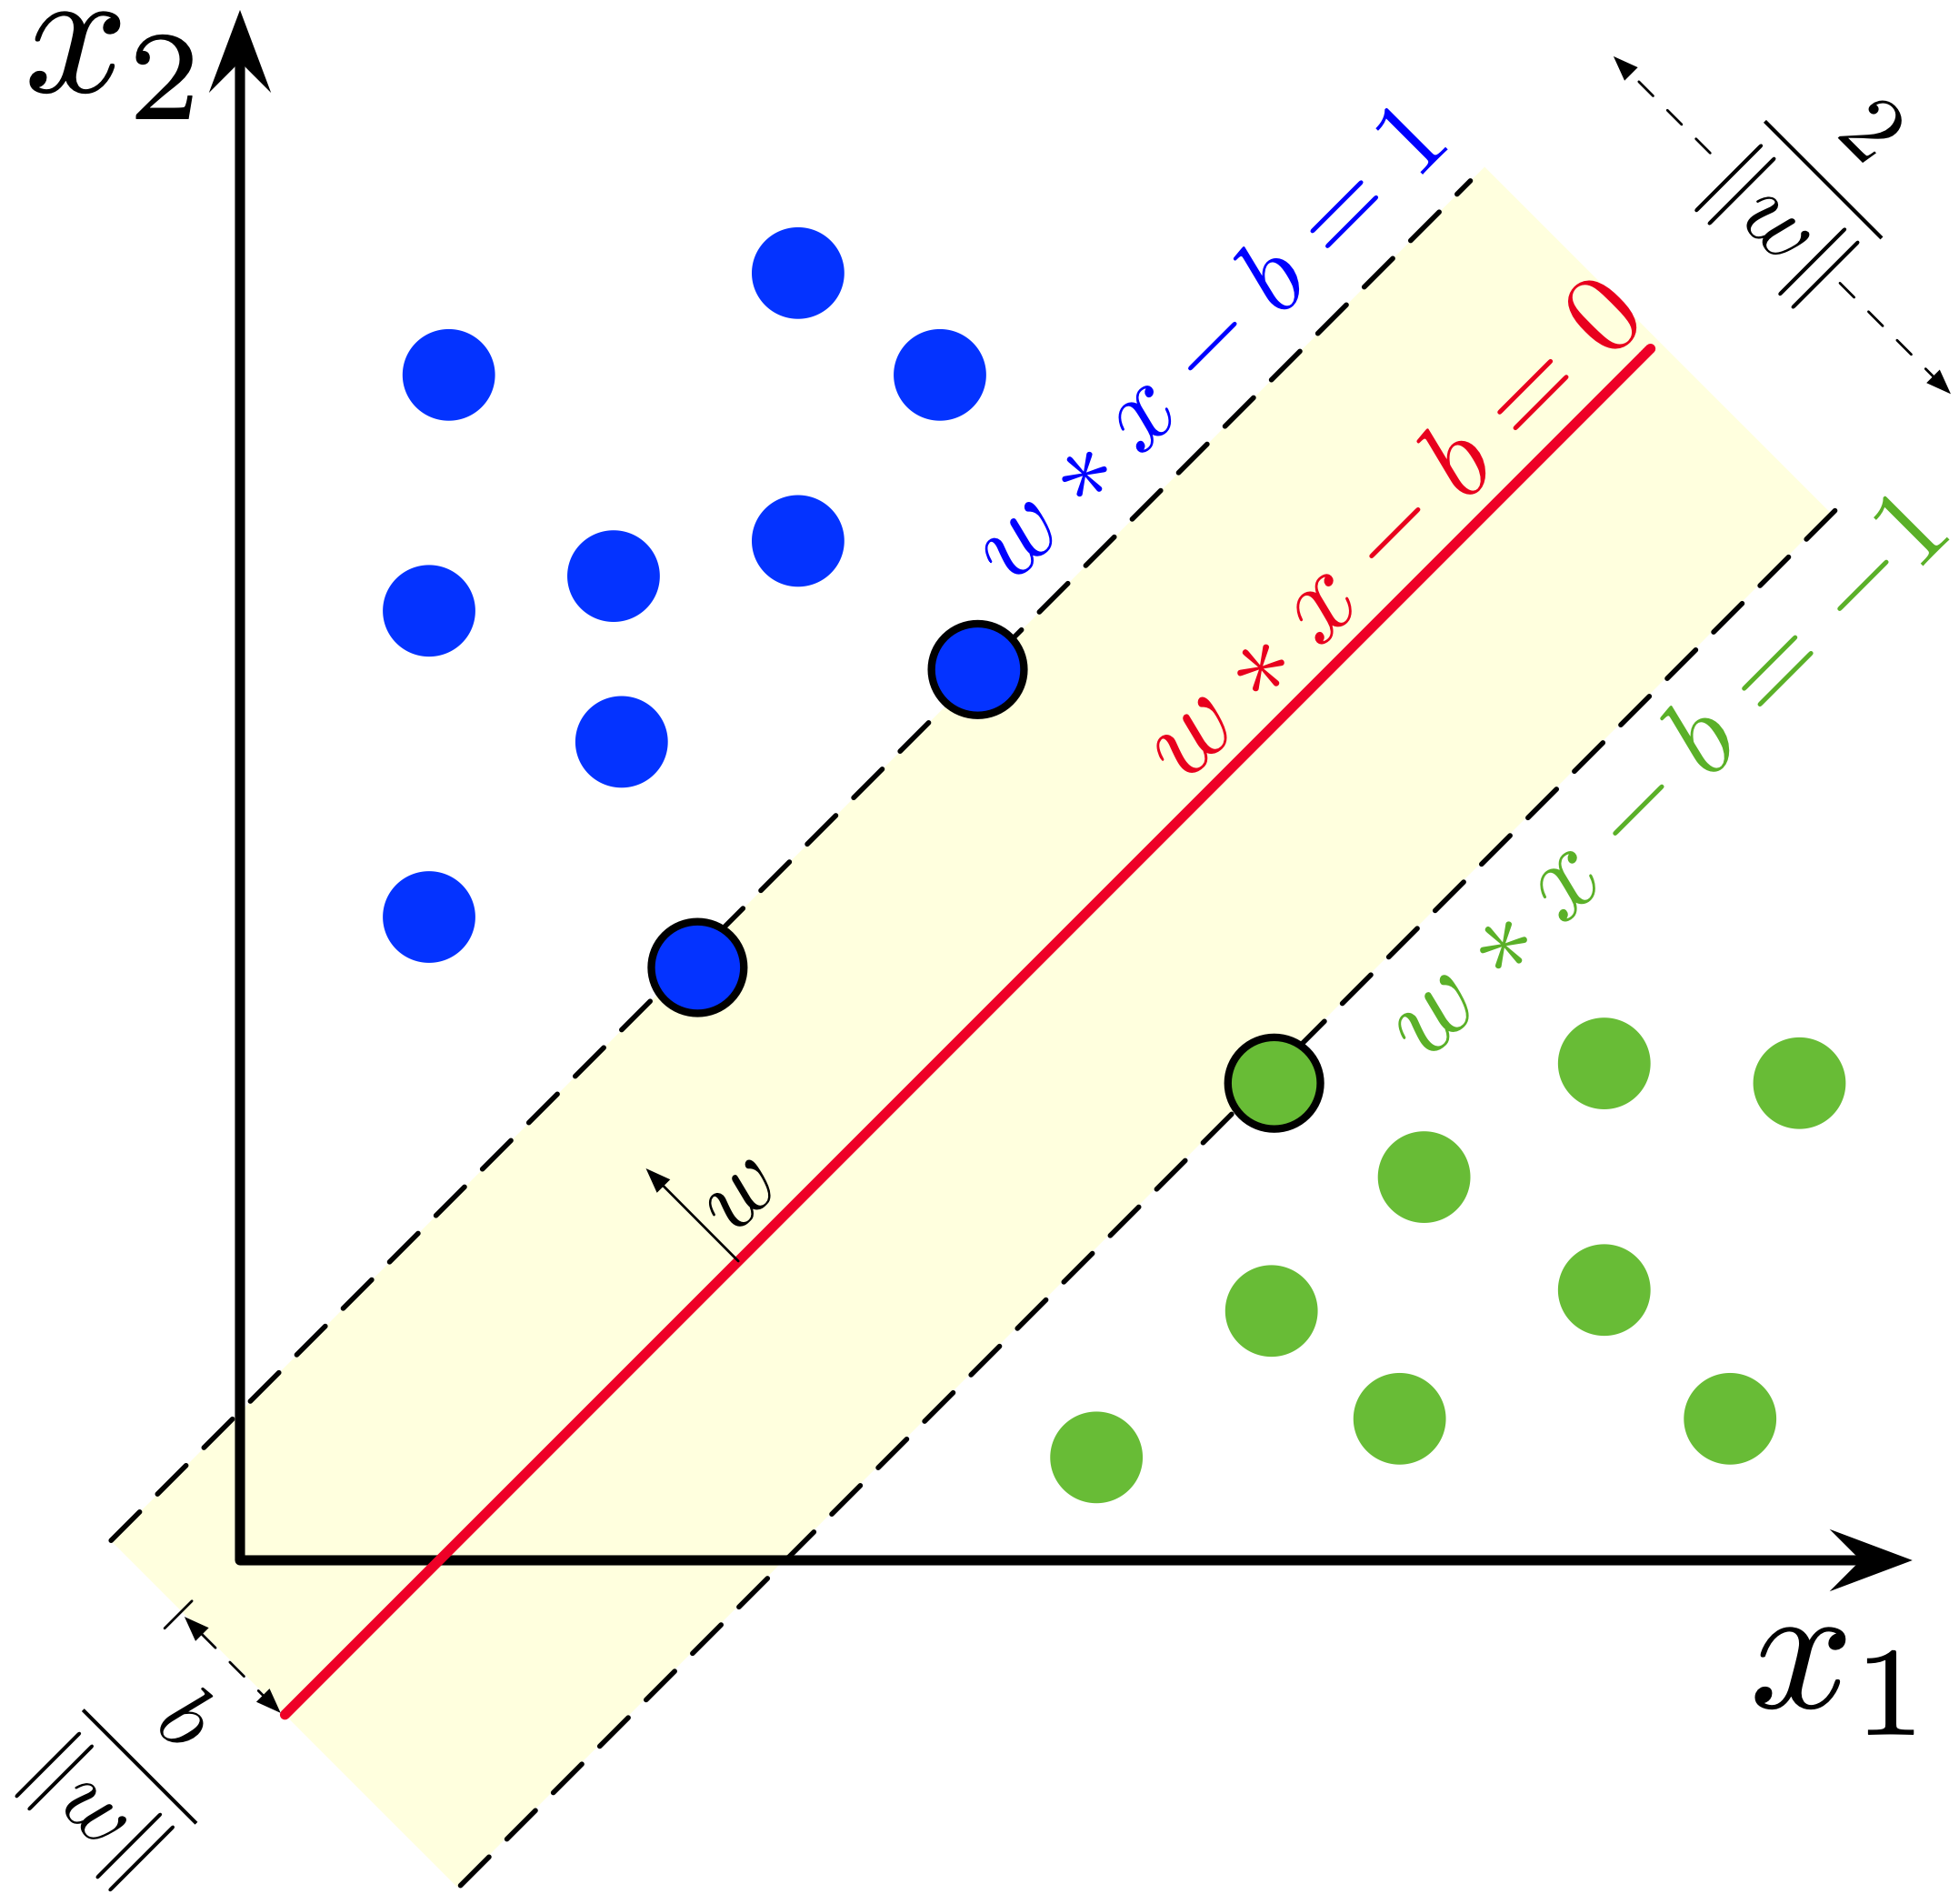
\includegraphics[width=0.4\textwidth]{SVM_margin.png}
	\end{center}
	\caption{Example graph showing a linear SVM classifier. 
	Image licensed under the Creative Commons Attribution-Share Alike 4.0 International \cite{larhmam}}
    \label{fig:svm}
\end{figure}

Figure~\ref{fig:svm} shows a linear SVM classifier. Linearly separable problems can be separated using the function:

\begin{equation}
	f(\textbf{x}) = \textbf{w} * \textbf{x} + b
\end{equation}

Assuming a two-class problem, adding more classes simply adds more dimensions. However, there will be many possible lines that fulfil this separation. We must select the best line. 

$\gamma_{i}$ is the distance between a point $x_i$ and the hyperplane $\textbf{w} * \textbf{x}_{i} + b = 0$:

\begin{equation}
	\gamma_{i} = \frac{t_{i}(\textbf{w} * \textbf{x}_{i} + b)}{\left|\left|\textbf{w}\right|\right|}
\end{equation}

$\gamma$ is the distance between the hyperplane and the \textit{nearest point} in each class. Let:

$$ t_{i}(\textbf{w} * \textbf{x}_{i} + b) \ge 1 $$

Yields:

\begin{equation}
	\gamma = \min_i \gamma_i = \frac{1}{\left|\left|\textbf{w}\right|\right|}
\end{equation}

The data points that define the hyperplane, the ones that lie on the margins, are called the \textit{support vectors}. These points have black edges in Figure~\ref{fig:svm}. Thus our \textit{optimisation problem}, to find the maximum $\gamma$, is defined as:

\begin{equation}
	 \max_{\textbf{w}, b} \gamma = \max_{\textbf{w}, b}\frac{1}{\left|\left|\textbf{w}\right|\right|} \Rightarrow \min_{\textbf{w}, b}\textbf{w}^{T}\textbf{w}
\end{equation}

Subject to:

$$ t_{i}(\textbf{w} * \textbf{x}_{i} + b) \ge 1, \forall i $$

There are a number of solving the optimisation problem. A Bayesian method would be to simply take the average of all possible functions. Another, more formal, way of doing this is to use the method of \textit{Lagrange multipliers}. Our Lagrangian function is:

\begin{equation}
	\Lagr(\textbf{w}, b, \alpha) = \frac{1}{2}\textbf{w}^{T}\textbf{w} = \sum^{n}_{i=1} \alpha_{i}(t_{i}(\textbf{w} * \textbf{x}_{i} + b)-1)
\end{equation}

Where $\alpha_{i} \ge 0 (\forall i \in 1, 2, ..., n)$ are the Lagrange multipliers. Now we can use the differential to find the optimization:

\begin{equation}
	\frac{\partial\Lagr(\textbf{w}, b, \alpha)}{\partial{\textbf{w}}} = \textbf{w} - \sum^{n}_{i=1} \alpha_{i}t_{i}\textbf{x}_{i} = 0
\end{equation}

\begin{equation}
	\frac{\partial\Lagr(\textbf{w}, b, \alpha)}{\partial{b}} = - \sum^{n}_{i=1} \alpha_{i}t_{i} = 0
\end{equation}

Substituting gives us the \textit{dual optimization problem}- maximize:

\begin{equation}
	\Lagr(\alpha) = \sum^{n}_{i=i} \alpha_{i} - \frac{1}{2}\sum^{n}_{i,j=i} \alpha_{i}\alpha_{j}t_{i}t_{j}(\textbf{x}_{i} * \textbf{x}_{j})
\end{equation}

Subject to $ \alpha_{i} \ge 0 \forall i $ and $ \sum^{n}_{i=1} \alpha_{i}t_{i} = 0 $

This is a quadratic function, and is therefore easily solvable.

Very few problems are completely separable, however. We can use a variable $\zeta$ to allow for misclassification errors this turns the optimization problem into:

\begin{equation}
	\min_{\textbf{w}, b} \textbf{w}^{T}\textbf{w} + C \sum^{n}_{i=1} \zeta_{i}
\end{equation}

Subject to:

$$ t_{i}(\textbf{w} * \textbf{x}_{i} + b) \ge 1 - \zeta_{i}, \forall i \in 1, 2, 3, ..., n $$

And:

$$ \zeta_{i} \ge 0, \forall i \in 1, 2, 3, ..., n $$

This is called a `soft margin', since $\zeta$ allows points past the margin. $C$ is a regularisation argument- a small $C$ allows more points past the margin. A small $C$ reduces the number of points past the margin.

The above method is the traditional method for solving support vector classifiers. There are more modern algorithms now available. For example sub-gradient descent algorithms \cite{bertsekas}, \cite{shor} have also been used in the context of SVMs, and have shown to be more efficient \cite{cotter}. A coordinate descent approach has been used too \cite{hsieh}.

In the context of image classification, the original SVM paper authors used their SVM for handwriting classifiers \cite{bottou}. This paper is especially useful for comparing SVMs against other classifiers, for example kNNs and CNNs, despite the simple training dataset.

\subsubsection{CNNs}
Convolutional Neural Networks (CNNs) are now the main classification system used for image classification. A the core of the CNN there is the perceptron, which has already been discussed here. \cite{minsky} is a famous book that stalled the use and development of perceptrons for many years; but what came next is using multiple layers of perceptrons, through which data travels and is transformed with each level. To train a CNN we must have some measure of the accuracy of the fit, for example by using the sum of squares error:

\begin{equation}
	E = \frac{1}{2} \sum^{N}_{n=1} \sum^{c}_{k=1} (y_{k} (\textbf{x}^{n}; \textbf{w}) - t_{k}^{n})^2
\end{equation}

Where $y_k$ is the $k^{th}$ output and $t_{k}^{n}$ is the target output for the $n^{th}$ training data of the $\textbf{x}^{n}$ corrisponding input data.

We iteratively update the value of $\textbf{w}$ which minimizes the error $E$ with the \textit{gradient descent}- the derivative of $E$. This is called the \textit{back-propagation algorithm}.

In the context of computer vision, CNNs can be used to form position independent filters to extract features. 

\section{Evaluation}
\subsection{Tiny Images}
Our implementation of tinyimages had three tunable parameters: the number of vertical pixels to crop to, the colour space to use, and the cropping algorithm. The colour space options were \texttt{rgb} and \texttt{grayscale}. The cropping algorithms were \texttt{crop} and \texttt{distort}. \texttt{crop} cuts out the center of the image so that it is always a square. \texttt{distort} distorts aspect ratio to a square.

Evaluation was done using the same training and test datasets, and on the same classifier (the default one) for fairness:

\begin{figure}[H]
	\begin{center}
		\begin{tikzpicture}
			\begin{groupplot}[
				group style={
					columns=3,rows=4,
					horizontal sep=1.5cm,
					vertical sep=1.5cm
				}]
				\nextgroupplot[
						width=0.24\textwidth,
						axis y line*=left,
						title={Grayscale and Crop},
						xmin=0, xmax=100,
						ymin=0, ymax=0.4
					] % 1
					\addplot[
						only marks,
		    			color=red,
		    			mark size=0.5pt
		    		] 
		    		table[x=imsize,y=accuracy,col sep=comma] {../code/results_csv/tinyimages_grayscale_crop.csv};
				\nextgroupplot[
						at=(group c1r1.west),
						width=0.24\textwidth,
						axis y line*=right,
		  				axis x line=none,
						xmin=0, xmax=100,
						ymin=14, ymax=20
					] % 1, 2nd axis
					\addplot[
						only marks,
		    			color=black,
		    			mark size=0.5pt
		    		] 
		    		table[x=imsize,y=time,col sep=comma] {../code/results_csv/tinyimages_grayscale_crop.csv};
				\nextgroupplot[
						width=0.24\textwidth,
						axis y line*=right,
		  				axis x line=none,
						xmin=0, xmax=100,
						ymin=14, ymax=20
			        ] % 2, 2nd axis
					\addplot[
						only marks,
		    			color=black,
		    			mark size=0.5pt
		    		] 
		    		table[x=imsize,y=time,col sep=comma] {../code/results_csv/tinyimages_grayscale_distort.csv};
				\nextgroupplot[width=0.2\textwidth,at=(group c3r1.north),
			    		width=0.24\textwidth,
						axis y line*=left,
						title={Grayscale and Distort},
						xmin=0, xmax=100,
						ymin=0, ymax=0.4,
			        ]
					\addplot[
						only marks,
		    			color=red,
		    			mark size=0.5pt
		    		] 
		    		table[x=imsize,y=accuracy,col sep=comma] {../code/results_csv/tinyimages_grayscale_distort.csv};
		    \end{groupplot}
		 \end{tikzpicture}
		 \begin{tikzpicture}
		    \begin{groupplot}[
				group style={
					columns=3,rows=4,
					horizontal sep=1.5cm,
					vertical sep=1.5cm
				}]
		    	\nextgroupplot[
						width=0.24\textwidth,
						axis y line*=left,
						title={RGB and Crop},
						xmin=0, xmax=100,
						ymin=0, ymax=0.4
					] % 1
					\addplot[
						only marks,
		    			color=red,
		    			mark size=0.5pt
		    		] 
		    		table[x=imsize,y=accuracy,col sep=comma] {../code/results_csv/tinyimages_rgb_crop.csv};
		    		\nextgroupplot[
						at=(group c1r1.west),
						width=0.24\textwidth,
						axis y line*=right,
		  				axis x line=none,
						xmin=0, xmax=100,
						ymin=14, ymax=20
					] % 1, 2nd axis
					\addplot[
						only marks,
		    			color=black,
		    			mark size=0.5pt
		    		] 
		    		table[x=imsize,y=time,col sep=comma] {../code/results_csv/tinyimages_rgb_crop.csv};
		    	\nextgroupplot[
						width=0.24\textwidth,
						axis y line*=right,
		  				axis x line=none,
						xmin=0, xmax=100,
						ymin=14, ymax=20,
						legend style={
					    	at={(0.0,-0.25)},
							anchor=north,
						}						
			        ] % 2, 2nd axis
					\addplot[
						only marks,
		    			color=black,
		    			mark size=0.5pt
		    		] 
		    		table[x=imsize,y=time,col sep=comma] {../code/results_csv/tinyimages_rgb_distort.csv};
		    		\addlegendentry{Time [Seconds]}
				\nextgroupplot[width=0.2\textwidth,at=(group c3r1.north),
			    		width=0.24\textwidth,
						axis y line*=left,
						title={RGB and Distort},
						xmin=0, xmax=100,
						ymin=0, ymax=0.4,
						legend style={
					    	at={(0.9,-0.25)},
							anchor=north,
						},
			        ]
					\addplot[
						only marks,
		    			color=red,
		    			mark size=0.5pt
		    		] 
		    		table[x=imsize,y=accuracy,col sep=comma] {../code/results_csv/tinyimages_rgb_distort.csv};
		    		\addlegendentry{Accuracy}
			\end{groupplot}
		\end{tikzpicture}
	\end{center}
	\caption{Graphs showing classifier accuracy (left axis) and time taken (right axis) for resizing to a given number of pixels (tinyimages), in different colour spaces, and using different cropping algorithms} 
    \label{fig:tinyimages}
\end{figure}

\subsubsection{Resizing Images}
Figure~\ref{fig:tinyimages} shows that distorting the images lead to better accuracy than cropping them. A hypothesis for this could be that less pixel information is lost this way. 

\subsubsection{Colours}
Figure~\ref{fig:tinyimages} also shows that using an RGB colour space leads to significantly better accuracy, with no speed penalty. Indeed, the \textit{most accurate} parameters were also the \textit{fastest}!

\subsubsection{Image Sizes}
These tests show that adding more pixels does not mean more accuracy. For all tests, the best accuracy is from 4-16 vertical pixels. Accuracy tapers off after that.

The best accuracy was achieved resizing to five vertical pixels, distorting the image, using the RGB colour space, with an accuracy using the default classifier of 0.332.



\subsection{Colour Histograms}

Our implementation of colour histograms had two tunable parameters. The number of bins for the histogram to use and the colour space to use. Tests and their conclusions are shown below:

\begin{figure}[H]
    \centering
	\begin{tikzpicture}
		\begin{axis}[
			axis y line*=left,
		    title={Accuracy as a function of the number of histogram bins},
		    xlabel={Number of Histogram Bins},
		    ylabel={Accuracy},
		    xmin=0, xmax=256,
		    ymin=0, ymax=0.4,
		    legend style={
		    	at={(0.25,-0.2)},
				anchor=north,
			},
		    ymajorgrids=true,
		    grid style=dashed,
		]
		
		\addplot[
		    	only marks,
		    	color=red,
		    	mark size=0.5pt
		    ]
		    table[x=numbins,y=accuracy,col sep=comma] {../code/results_csv/colourhistograms_rgb.csv};
		    %\legend{RGB}
		    \addlegendentry{RGB Accuracy}
		\addplot[
		    	only marks,
		    	color=blue,
		    	mark size=0.5pt
		    ]
		    table[x=numbins,y=accuracy,col sep=comma] {../code/results_csv/colourhistograms_grayscale.csv};
		    %\legend{Grayscale}
		    \addlegendentry{Grayscale Accuracy}
		    
		\end{axis}
		
		\pgfplotsset{every axis y label/.append style={rotate=180,yshift=8.8cm}}
		\begin{axis}[
			axis y line*=right,
		  	axis x line=none,
		  	ymin=0, ymax=100,
		  	xmin=0, xmax=256,
		  	ylabel={Time [Seconds]},
		  	legend style={
		    	at={(0.75,-0.2)},
				anchor=north,
			},
		]
		\addplot[
				only marks,
		    	color=black,
		    	mark size=0.5pt
			] 
			table[x=numbins,y=time,col sep=comma] {../code/results_csv/colourhistograms_rgb.csv};
			\addlegendentry{RGB Time}
		\addplot[
				only marks,
		    	color=gray,
		    	mark size=0.5pt
			] 
			table[x=numbins,y=time,col sep=comma] {../code/results_csv/colourhistograms_grayscale.csv};
			\addlegendentry{Grayscale Time}
		\end{axis}
	\end{tikzpicture}
	\caption{Graph showing resulting classifier accuracy, and the time taken, from the number of histogram bins and colour space used} 
    \label{fig:colourhistograms}
\end{figure}


\subsubsection{Quantisation}
Image quantisation defines into how many bins there are in the histogram there are. My testing showed that the ideal number of bins was 10, which gave me an accuracy of 0.326, using the default classifier. There was no noticeable time penalty for using more bins.

\subsubsection{Colour Spaces}
We can either convert to grayscale and make just one histogram, or we can make three histograms, one for each colour channel, and them vectorize them. My testing showed that doing the latter led to much better accuracy, which a negligible time increase.

\subsection{kNN classifier}
\subsubsection{K value}
Our implementation of a kNN classifier has four tunable parameters:

\begin{itemize}
	\item The value of $k$ (the number of nearest points to consider)
	\item The distance function to use
	\item The voting method (how a result is produced from $k$ different results)
	\item The average function to use (two voting methods require averaging)
\end{itemize}

\begin{figure}[H]
    \centering
	\begin{tikzpicture}
		\begin{groupplot}[
			group style={
				columns=3,rows=4,
				horizontal sep=1.5cm,
				vertical sep=1.5cm
			}]
			\nextgroupplot[
				width=0.24\textwidth,
			    title={Best Histograms},
			    ylabel={Accuracy},
			    xmin=0, xmax=100,
			    ymin=0, ymax=0.4,
			    ymajorgrids=true,
			    grid style=dashed,
			]		
			\addplot[
			    	only marks,
			    	color=green,
			    	mark size=0.5pt
			    ]
			    table[x=k,y=majorityvote accuracy,col sep=comma] {../code/results_csv/knn_best_histograms_euclidean.csv};
			    %\legend{RGB}
			\addplot[
			    	only marks,
			    	color=red,
			    	mark size=0.5pt
			    ]
			    table[x=k,y=averageminimumdistance mean accuracy,col sep=comma] {../code/results_csv/knn_best_histograms_euclidean.csv};
			    %\legend{Grayscale}
		    \addplot[
		    	only marks,
		    	color=orange,
		    	mark size=0.5pt
		    ]
		    table[x=k,y=averageminimumdistance median accuracy,col sep=comma] {../code/results_csv/knn_best_histograms_euclidean.csv};
		    %\legend{Grayscale}
		    \addplot[
		    	only marks,
		    	color=blue,
		    	mark size=0.5pt
		    ]
		    table[x=k,y=weightedmajorityvote mean accuracy,col sep=comma] {../code/results_csv/knn_best_histograms_euclidean.csv};
		    %\legend{Grayscale}
		    \addplot[
		    	only marks,
		    	color=cyan,
		    	mark size=0.5pt
		    ]
		    table[x=k,y=weightedmajorityvote median accuracy,col sep=comma] {../code/results_csv/knn_best_histograms_euclidean.csv};
		    %\legend{Grayscale}
		    \nextgroupplot[
			    width=0.24\textwidth,
			    title={Best Tinyimages},
			    xmin=0, xmax=100,
			    ymin=0, ymax=0.4,
			    legend style={
			    	at={(0.25,-0.2)},
					anchor=north,
				},
			    ymajorgrids=true,
			    grid style=dashed,
			]		
			\addplot[
			    	only marks,
			    	color=green,
			    	mark size=0.5pt
			    ]
			    table[x=k,y=majorityvote accuracy,col sep=comma] {../code/results_csv/knn_best_tinyimages_euclidean.csv};
			    %\legend{RGB}
			\addplot[
			    	only marks,
			    	color=red,
			    	mark size=0.5pt
			    ]
			    table[x=k,y=averageminimumdistance mean accuracy,col sep=comma] {../code/results_csv/knn_best_tinyimages_euclidean.csv};
			    %\legend{Grayscale}
		    \addplot[
		    	only marks,
		    	color=orange,
		    	mark size=0.5pt
		    ]
		    table[x=k,y=averageminimumdistance median accuracy,col sep=comma] {../code/results_csv/knn_best_tinyimages_euclidean.csv};
		    %\legend{Grayscale}
		    \addplot[
		    	only marks,
		    	color=blue,
		    	mark size=0.5pt
		    ]
		    table[x=k,y=weightedmajorityvote mean accuracy,col sep=comma] {../code/results_csv/knn_best_tinyimages_euclidean.csv};
		    %\legend{Grayscale}
		    \addplot[
		    	only marks,
		    	color=cyan,
		    	mark size=0.5pt
		    ]
		    table[x=k,y=weightedmajorityvote median accuracy,col sep=comma] {../code/results_csv/knn_best_tinyimages_euclidean.csv};
		    %\legend{Grayscale}
		\end{groupplot}
	\end{tikzpicture}
	\begin{tikzpicture}
		\begin{groupplot}[
			group style={
				columns=3,rows=4,
				horizontal sep=1.5cm,
				vertical sep=1.5cm
			}]
			\nextgroupplot[
				width=0.24\textwidth,
			    xlabel={Value of $k$},
			    ylabel={Time [Seconds]},
			    xmin=0, xmax=100,
			    ymin=0, ymax=4,
			    ymajorgrids=true,
			    grid style=dashed,
			]		
			\addplot[
			    	only marks,
			    	color=green,
			    	mark size=0.5pt
			    ]
			    table[x=k,y=majorityvote time,col sep=comma] {../code/results_csv/knn_best_histograms_euclidean.csv};
			    %\legend{RGB}
			\addplot[
			    	only marks,
			    	color=red,
			    	mark size=0.5pt
			    ]
			    table[x=k,y=averageminimumdistance mean time,col sep=comma] {../code/results_csv/knn_best_histograms_euclidean.csv};
			    %\legend{Grayscale}
		    \addplot[
		    	only marks,
		    	color=orange,
		    	mark size=0.5pt
		    ]
		    table[x=k,y=averageminimumdistance median time,col sep=comma] {../code/results_csv/knn_best_histograms_euclidean.csv};
		    %\legend{Grayscale}
		    \addplot[
		    	only marks,
		    	color=blue,
		    	mark size=0.5pt
		    ]
		    table[x=k,y=weightedmajorityvote mean time,col sep=comma] {../code/results_csv/knn_best_histograms_euclidean.csv};
		    %\legend{Grayscale}
		    \addplot[
		    	only marks,
		    	color=cyan,
		    	mark size=0.5pt
		    ]
		    table[x=k,y=weightedmajorityvote median time,col sep=comma] {../code/results_csv/knn_best_histograms_euclidean.csv};
		    %\legend{Grayscale}
		    \nextgroupplot[
			    width=0.24\textwidth,
			    xlabel={Value of $k$},
			    xmin=0, xmax=100,
			    ymin=0, ymax=4,
			    legend style={
			    	at={(-0.25,-0.5)},
					anchor=north,
				},
			    ymajorgrids=true,
			    grid style=dashed,
			]		
			\addplot[
			    	only marks,
			    	color=green,
			    	mark size=0.5pt
			    ]
			    table[x=k,y=majorityvote time,col sep=comma] {../code/results_csv/knn_best_tinyimages_euclidean.csv};
			    %\legend{RGB}
			    \addlegendentry{\texttt{majorityvote}}
			\addplot[
			    	only marks,
			    	color=red,
			    	mark size=0.5pt
			    ]
			    table[x=k,y=averageminimumdistance mean time,col sep=comma] {../code/results_csv/knn_best_tinyimages_euclidean.csv};
			    %\legend{Grayscale}
			    \addlegendentry{\texttt{averageminimumdistance mean}}
		    \addplot[
		    	only marks,
		    	color=orange,
		    	mark size=0.5pt
		    ]
		    table[x=k,y=averageminimumdistance median time,col sep=comma] {../code/results_csv/knn_best_tinyimages_euclidean.csv};
		    %\legend{Grayscale}
		    \addlegendentry{\texttt{averageminimumdistance median}}
		    \addplot[
		    	only marks,
		    	color=blue,
		    	mark size=0.5pt
		    ]
		    table[x=k,y=weightedmajorityvote mean time,col sep=comma] {../code/results_csv/knn_best_tinyimages_euclidean.csv};
		    %\legend{Grayscale}
		    \addlegendentry{\texttt{weightedmajorityvote mean}}
		    \addplot[
		    	only marks,
		    	color=cyan,
		    	mark size=0.5pt
		    ]
		    table[x=k,y=weightedmajorityvote median time,col sep=comma] {../code/results_csv/knn_best_tinyimages_euclidean.csv};
		    %\legend{Grayscale}
		    \addlegendentry{\texttt{weightedmajorityvote median}}
	
		\end{groupplot}
	\end{tikzpicture}
	\caption{Graphs showing resulting accuracy, and the time taken, from the value of $k$ with different averaging functions, using the \textbf{euclidean} distance function} 
    \label{fig:knn_euclidean}
\end{figure}

\subsubsection{Value of $k$}
The value of $K$ selects from how many nearest neighbours are considered. For the majority vote and weighted majority vote, the peak accuracy was a $k$ of around 20. The time taken seemed to increase proportionally, but not linear-ally, as $k$ increases. Here the relative increase is important, since tests were done on a number of different computers.

\subsubsection{Voting Algorithm}
When we consider $k$ nearest neighbours, we must decide from which of them we make a prediction. The simplest possible way to do this is just a majority vote, which is implemented in our code using the \texttt{majorityvote} parameter. \cite{dudani} describes how this is not ideal, since it does not consider the individual distances of the $k$ nearest neighbours. It suggests two improvements: weighing the votes by a factor of the distance, and weighing the votes by the rank of the distance. We only implemented the former of these, using the \texttt{weightedmajorityvote} argument. We want the \textit{smallest} distance to have the \textit{largest} multiplier- \cite{dudani}  achieves this by multiplying by the inverse of the distance:

$$ w_{x} = \frac{1}{D(x, y)} $$

We achieve this by subtracting each distance by the largest distance and taking the magnitude:

$$ \textbf{d}_{2} = \left| \textbf{d}_{1}  - \max(\textbf{d}_{1}) \right| $$

The final algorithm selects the label with the lowest average distance from the point.

The latter two algorithms need a definition for `average' so we here have two additional options: to use the median or the mean.

Figure~\ref{fig:knn_euclidean} shows that for all values of $k$, using a weighted majority vote was slightly more accurate than using a simple majority vote. Using the average minimum distance, the accuracy decreased as $k$ increased. This leads me to believe that it is not a good algorithm.

For all tests, using the mean was more accurate than using the median. Generally for statistics we prefer to use the median since it is less distorted by extreme results, but in this context this is something we want.

These conclusions were the same for both colour histograms and tiny images, this is also shown in Figure~\ref{fig:knn_euclidean}.

\subsubsection{Distance Measurement Algorithm}

\begin{figure}[H]
	\begin{center}
		\begin{tikzpicture}
			\begin{axis}[
					ymin=0, ymax=0.4,
					xtick=data,
% 					nodes near coords,
					ylabel = {Highest accuracy achieved},
					symbolic x coords = {chebychev, cityblock, correlation, euclidean, hamming, jaccard, mahalanobis, minkowski},
					xticklabel style={rotate=90},
					bar width=4pt,
					legend style={
		    			at={(0.5,-0.4)},
						anchor=north,
					},
				]
				\addplot[
					bar shift = -3pt,
					ybar,
					fill=blue
				]
				table[x=metric,y=accuracy,col sep=comma] {../code/results_csv/best_tinyimages.csv};
				\addlegendentry{tinyimages}
				\addplot[
					bar shift = +3pt,
					ybar,
					fill=red
				]
				table[x=metric,y=accuracy,col sep=comma] {../code/results_csv/best_histograms.csv};
				\addlegendentry{histograms}
				%\legend{tinyimages, histograms}				
			\end{axis}
		\end{tikzpicture}
	\end{center}
	\caption{Chart showing maximum accuracies achieved with different distance metrics}
	\label{fig:distancemetrics}
\end{figure}

There are a number of different metrics we can use to define distance between points. Figure~\ref{fig:distancemetrics} shows the different performances of these algorithms. For histograms, \texttt{cityblock}, \texttt{euclidean} and \texttt{minkowski} are tied at having the best preformance, but \texttt{euclidean} and \texttt{minkowski} are considered superior since they achieved this with a smaller value of $k$: (20 vs. 17). For tinyimages, the \texttt{correlation} metric was the best, with a value of 37 for $k$.

\subsection{Other metrics}
So far we have only considered the accuracy as a metric of performance. This can potentially be dangerous. A confusion matrix can be used to show us more detail, the true positives, false positives, false negatives, and true negatives:

\begin{table}[H]
	\begin{center}
		\begin{tabular}{ll|ll}
			                           &          & \multicolumn{2}{c}{Actual}      \\
			                           &          & Positive       & Negative       \\
			\midrule 
			\multirow{2}{*}{Predicted} & Positive & True Positive  & False Positive \\
			                           & Negative & False Negative & True Negative  \\
		\end{tabular}
	\end{center}
\end{table}

From this data we can calculate additional metrics.

\begin{figure}[H]
	\begin{center}
		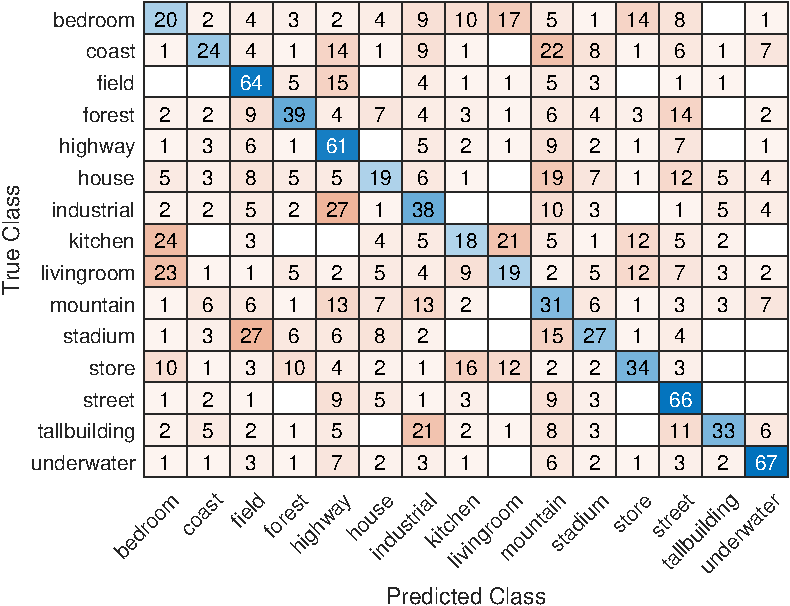
\includegraphics[width=0.4\textwidth]{tinyimages_confusionmatrix.pdf}
	\end{center}
    \caption{Confusion Matrix, generated from best \textbf{tinyimages} parameters.}
    \label{fig:tinyimages_confusionmatrix}
\end{figure}

\begin{figure}[H]
	\begin{center}
		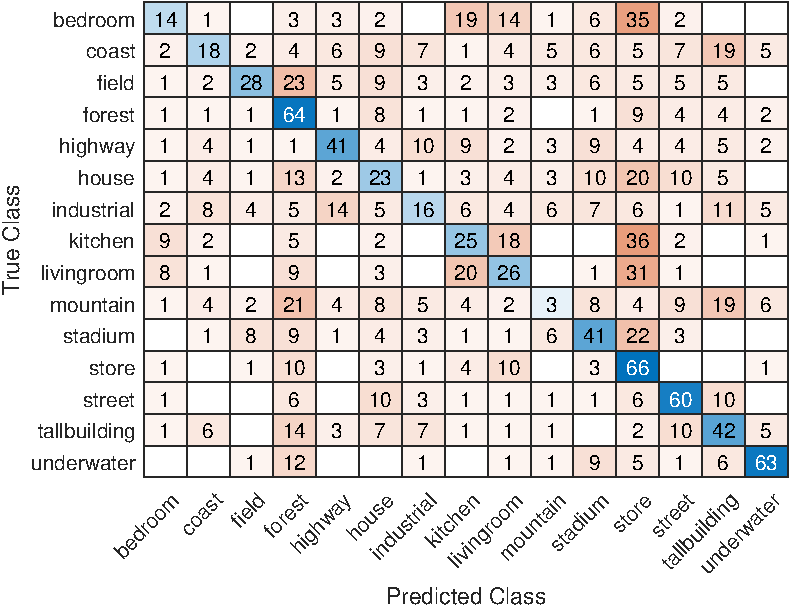
\includegraphics[width=0.4\textwidth]{histograms_confusionmatrix.pdf}
	\end{center}
    \caption{Confusion Matrix, generated from best \textbf{histograms} parameters.}
    \label{fig:tinyimages_histograms}
\end{figure}

Since our classifier can predict multiple outcomes besides true and false, we add columns to show incorrect predictions. Figure~\ref{fig:tinyimages_confusionmatrix} shows the confusion matrix for tinyimages. The diagonal line is correct predictions. The \textit{true positive rate}, also called the \textit{sensitivity} or \textit{recall}, is the proportion of predictions correctly classified; it is given by:

$$ \mbox{True Positive Rate} = \frac{\mbox{True Positives}}{\mbox{True Positives} \times \mbox{False Negatives}} $$

Conversely, the \textit{true negative rate}, also called the \textit{specificity} is the proportion of negative cases that were correctly classified. It is given by:

$$ \mbox{True Negative Rate} = \frac{\mbox{True Negatives}}{\mbox{False Positives} \times \mbox{True Negatives}} $$

We also have the \textit{false positive rate}, also called the \textit{type I error}:

$$ \mbox{False Positive Rate} = \frac{\mbox{False Positives}}{\mbox{False Positives} \times \mbox{True Negatives}} $$

and the \textit{false negative rate}, also called the \textit{type II error}:

$$ \mbox{False Negative Rate} = \frac{\mbox{False Negatives}}{\mbox{True Positives} \times \mbox{False Negatives}} $$

Plotting the False Positive Rate against the True Positive Rate gives us the \textit{Receiver Operator Curve} (ROC). The area under the ROC can be an important metric.

The \textit{balanced accuracy} is an important metric if many more predictions should be from one class than another; e.g. medical testing. It is given by:

$$ \mbox{Balanced Accuracy} = \frac{\mbox{True Positive Rate} + \mbox{True Negative Rate}}{2} $$

Table~\ref{table:metrics} shows metrics for different classifier labels and their averages.

\begin{table*}
	\begin{tabular}{r|cccccccccc}
	             & \multicolumn{2}{c}{sensitivity} & \multicolumn{2}{c}{specificity} & \multicolumn{2}{c}{precision} & \multicolumn{2}{c}{F}    & \multicolumn{2}{c}{Balanced Accuracy} \\
 & \rot{tinyimages} & \rot{histograms}  & \rot{tinyimages} & \rot{histograms}  & \rot{tinyimages} & \rot{histograms} & \rot{tinyimages} & \rot{histograms} & \rot{tinyimages} & \rot{histograms} \\
	\midrule
	bedroom      & 0.18        & 0.25        & 0.9636      & 0.9486      & 0.2609      & 0.2577     & 0.213       & 0.2538     & 0.5718            & 0.5993     \\
	coast        & 0.34        & 0.66        & 0.9664      & 0.8643      & 0.4198      & 0.2578     & 0.3757      & 0.3708     & 0.6532            & 0.76215    \\
	field        & 0.2         & 0.14        & 0.9471      & 0.9793      & 0.2128      & 0.3256     & 0.2062      & 0.1958     & 0.57355           & 0.55965    \\
	forest       & 0.19        & 0.26        & 0.9614      & 0.9521      & 0.2603      & 0.2796     & 0.2197      & 0.2694     & 0.5757            & 0.60605    \\
	highway      & 0.19        & 0.23        & 0.9671      & 0.9471      & 0.2923      & 0.2371     & 0.2303      & 0.2335     & 0.57855           & 0.58855    \\
	house        & 0.38        & 0.16        & 0.9379      & 0.97        & 0.304       & 0.2759     & 0.3378      & 0.2025     & 0.65895           & 0.565      \\
	industrial   & 0.27        & 0.41        & 0.9643      & 0.9521      & 0.3506      & 0.3796     & 0.3051      & 0.3942     & 0.61715           & 0.68105    \\
	kitchen      & 0.67        & 0.63        & 0.9757      & 0.9807      & 0.6634      & 0.7        & 0.6667      & 0.6632     & 0.82285           & 0.80535    \\
	livingroom   & 0.33        & 0.42        & 0.9843      & 0.94        & 0.6         & 0.3333     & 0.4258      & 0.3717     & 0.65715           & 0.68       \\
	mountain     & 0.66        & 0.6         & 0.9393      & 0.9579      & 0.4371      & 0.5042     & 0.5259      & 0.5479     & 0.79965           & 0.77895    \\
	stadium      & 0.61        & 0.41        & 0.9193      & 0.9721      & 0.3506      & 0.5125     & 0.4453      & 0.4556     & 0.76465           & 0.69105    \\
	store        & 0.64        & 0.28        & 0.9414      & 0.985       & 0.4384      & 0.5714     & 0.5203      & 0.3758     & 0.7907            & 0.6325     \\
	street       & 0.24        & 0.18        & 0.9779      & 0.9757      & 0.4364      & 0.3462     & 0.3097      & 0.2368     & 0.60895           & 0.57785    \\
	tallbuilding & 0.31        & 0.03        & 0.9121      & 0.9786      & 0.2013      & 0.0909     & 0.2441      & 0.0451     & 0.61105           & 0.5043     \\
	underwater   & 0.39        & 0.64        & 0.9707      & 0.9036      & 0.4875      & 0.3216     & 0.4333      & 0.4281     & 0.68035           & 0.7718     \\
	\midrule
	median       & 0.33        & 0.28        & 0.9636      & 0.9579      & 0.3506      & 0.3256     & 0.3378      & 0.3708     & 0.6532            & 0.6325     \\
	mean         & 0.3733 & 0.3533 & 0.9552 & 0.9538 & 0.3810 & 0.3595    & 0.3639 & 0.3362    & 0.6642     & 0.6535   
	\end{tabular}
	\caption{Table showing metrics for different classifier labels}
	\label{table:metrics}
\end{table*}

\subsection{Conclusion}
In conclusion, we have created an image classification system using non-CNN methods and have ran experiments to find the best parameters for this setup. However, the maximum accuracy we have achieved is ~0.4. All modern research in the area of image classification uses CNNs so we propose that using a CNN, in conjuncton with more advanced feature detection algorithms e.g. SIFT could achieve a much higher accuracy.


%\begin{table*}
%	\begin{center}
%		\begin{tabular}{@{}llllllllllllllll@{}}
%		\toprule
%		             & \rot{bedroom} & \rot{coast} & \rot{field} & \rot{forest} & \rot{highway} & \rot{house} & \rot{industrial} & \rot{kitchen} & \rot{livingroom} & \rot{mountain} & \rot{stadium} & \rot{store} & \rot{street} & \rot{tallbuilding} & \rot{underwater} \\ \midrule
%		bedroom      & 20      & 2     & 4     & 3      & 2       & 4     & 9          & 10      & 17         & 5        & 1       & 14    & 8      & 0            & 1          \\
%		coast        & 1       & 24    & 4     & 1      & 14      & 1     & 9          & 1       & 0          & 22       & 8       & 1     & 6      & 1            & 7          \\
%		field        & 0       & 0     & 64    & 5      & 15      & 0     & 4          & 1       & 1          & 5        & 3       & 0     & 1      & 1            & 0          \\
%		forest       & 2       & 2     & 9     & 39     & 4       & 7     & 4          & 3       & 1          & 6        & 4       & 3     & 14     & 0            & 2          \\
%		highway      & 1       & 3     & 6     & 1      & 61      & 0     & 5          & 2       & 1          & 9        & 2       & 1     & 7      & 0            & 1          \\
%		house        & 5       & 3     & 8     & 5      & 5       & 19    & 6          & 1       & 0          & 19       & 7       & 1     & 12     & 5            & 4          \\
%		industrial   & 2       & 2     & 5     & 2      & 27      & 1     & 38         & 0       & 0          & 10       & 3       & 0     & 1      & 5            & 4          \\
%		kitchen      & 24      & 0     & 3     & 0      & 0       & 4     & 5          & 18      & 21         & 5        & 1       & 12    & 5      & 2            & 0          \\
%		livingroom   & 23      & 1     & 1     & 5      & 2       & 5     & 4          & 9       & 19         & 2        & 5       & 12    & 7      & 3            & 2          \\
%		mountain     & 1       & 6     & 6     & 1      & 13      & 7     & 13         & 2       & 0          & 31       & 6       & 1     & 3      & 3            & 7          \\
%		stadium      & 1       & 3     & 27    & 6      & 6       & 8     & 2          & 0       & 0          & 15       & 27      & 1     & 4      & 0            & 0          \\
%		store        & 10      & 1     & 3     & 10     & 4       & 2     & 1          & 16      & 12         & 2        & 2       & 34    & 3      & 0            & 0          \\
%		street       & 1       & 2     & 1     & 0      & 9       & 5     & 1          & 3       & 0          & 9        & 3       & 0     & 66     & 0            & 0          \\
%		tallbuilding & 2       & 5     & 2     & 1      & 5       & 0     & 21         & 2       & 1          & 8        & 3       & 0     & 11     & 33           & 6          \\
%		underwater   & 1       & 1     & 3     & 1      & 7       & 2     & 3          & 1       & 0          & 6        & 2       & 1     & 3      & 2            & 67         \\ \bottomrule
%		\end{tabular}
%	\end{center}
%\end{table*}



\end{multicols}

% references aren't included in the pagecount :3
\pagebreak
\bibliographystyle{unsrt}
\bibliography{bibliography}

\end{document}